\documentclass{article}

\usepackage[a4paper, margin=1in]{geometry}
\usepackage[onehalfspacing]{setspace} % Correct 1.5 line spacing

\usepackage{graphicx}  % Figures
\graphicspath{{../figures/}}

\usepackage{fontspec}  % Fonts
\usepackage{helvet}
\usepackage{newpxtext,newpxmath}
\defaultfontfeatures{Scale=MatchLowercase, Ligatures=TeX}

\usepackage{url}
\usepackage[pdfusetitle]{hyperref}
\usepackage{titlesec}      % Modify title/section/chapter commands
\usepackage{mathtools}     % Various maths related commands
\usepackage{gensymb}       % \degree symbol
\usepackage[thinc]{esdiff} % Derivatives
\usepackage{booktabs}      % \toprule, etc., in tables

% https://tex.stackexchange.com/a/43009
\DeclarePairedDelimiter\abs{\lvert}{\rvert}%
\DeclarePairedDelimiter\norm{\lVert}{\rVert}%

% Caption figures
\usepackage{caption}
\DeclareCaptionFont{captionlabelfont}{\bfseries \sffamily}
\DeclareCaptionFont{captiontextfont}{\sffamily}
\captionsetup{labelfont=captionlabelfont, textfont=captiontextfont}

% Change footnote style
\renewcommand{\thefootnote}{\fnsymbol{footnote}}

% Fancy header/footer
\usepackage{fancyhdr}
\pagestyle{fancy}
\renewcommand{\sectionmark}[1]{\markright{\thesection . #1}}
\fancyhf{}
\lhead{\fancyplain{}{\thepage}}
\rhead{\fancyplain{}{\textit{\rightmark}}}

% Bibliography
\usepackage[backend=biber, style=phys, natbib=true,
			url=false, isbn=false, doi=false, eprint=false,
			autocite=superscript]{biblatex}

\addbibresource{references.bib}

\newcommand\mytitle    {Millimetre-Wave Cloud Profiling Radar}
\newcommand\mysubtitle {Pre-Project Review}
\newcommand\myauthor   {180014855}
\newcommand\mydate     {\today}
\newcommand\mymodule   {PH4111}
\newcommand\mywordcount{2000}

\title {\mytitle}
\author{\myauthor}
\date  {\mydate}

\begin{document}

\begin{titlepage}
	\centering
	{
\includegraphics[width=0.3\textwidth]{uos-logo}}
	\par
	{\LARGE\bfseries University of St. Andrews\par}
	{\LARGE School of Physics and Astronomy\par}
	\vspace{1.5cm}
	{\huge\bfseries\mytitle\par}
	{\Large\mysubtitle\par}
	\vspace{2cm}
	{\Large\myauthor\par}
	{\large\textbf{Module:} \mymodule\par}
	{\large\textbf{Word count:} \mywordcount\par}
	\vfill
	{\large\today\par}
\end{titlepage}

\begin{abstract}
This work is about \dots
\end{abstract}

\section{Introduction}
Meteorological radar systems provide great insight into weather phenomona, allowing for improved forecasts and for meteorologists to study clouds on a large scale. Clouds have a great influence on Earth's surface temperature, being able to both reflect and trap solar radiation, thus it is essential to study clouds to predict climate change. However, the high cost of conventional pulse Doppler radars limits deployment and hence the amount of cloud profling data that can be gathered.

Millimetre waves, particularly at 35 GHz and 94 GHz, are ideally suited to cloud radars due to their atmospheric attenuation properties \dots
Conventional pulse Doppler radars are expensive and require high peak power in contrast to frequency-modulated continuous wave (FMCW) radars, which require an average power potentially \dots less.
High carrier frequencies of FMCW radars allow for improved range and velocity resolution \dots


\section{Meteorological radar}
\subsection{Radar range equation}
The meteorological radar range equation relates the received and transmitted powers by 
\begin{equation}
	P_r = \frac{P_t G_t G_r \lambda^2}{(4 \pi)^3 r^4} \cdot \frac{\pi r^2 \theta \phi c \tau}{8} \cdot \frac{1}{2\ln{2}} \cdot \sum_{i=1}^N{\sigma_i} = \frac{P_t G_t G_r \lambda^2 \theta \phi c \tau}{1024 (\ln{2}) \pi^2 r^2} \sum_{i=1}^N{\sigma_i}, \label{eqn:MeteoRange}
\end{equation}
where \(P_r\) and \(P_t\) are the received and transmitted powers, \(G_r\) and \(G_t\) are receiver and transmitter attenna gains, \(\lambda\) is the carrier wavelength, \(r\) is the target range, \(\theta\) and \(\phi\) are the angular widths of the main lobe, \(\tau = 1/2B\), and \(\sigma_i\) is the radar cross-section (RCS) of target \(i\).
The first term is simply the radar range equation for a point target. The second term is the volume sampled by the radar. The third term is a correction derived by Probert-Jones in 1962, arising from the non-uniform gain profile.\supercite{ProbertJones} The last term accounts for the number of particles and their individual radar cross-sections.

In the Rayleigh scattering regime, the RCS takes the form
\begin{align}
	\sigma_i = \frac{\pi^5}{\lambda^4} D_i^6 \abs{K}^2 &&
	\abs{K}^2 \approx \begin{cases}
		0.93  & \text{water phase}, \\
		0.197 & \text{ice phase},   \\
	\end{cases}\label{eqn:RCS}
\end{align}
where \(D_i\) is the \(i\)th drop diameter.\supercite{RadarHandbookMeteoRange}

\subsection{Frequency-modulated continuous wave radar}
\begin{figure}
	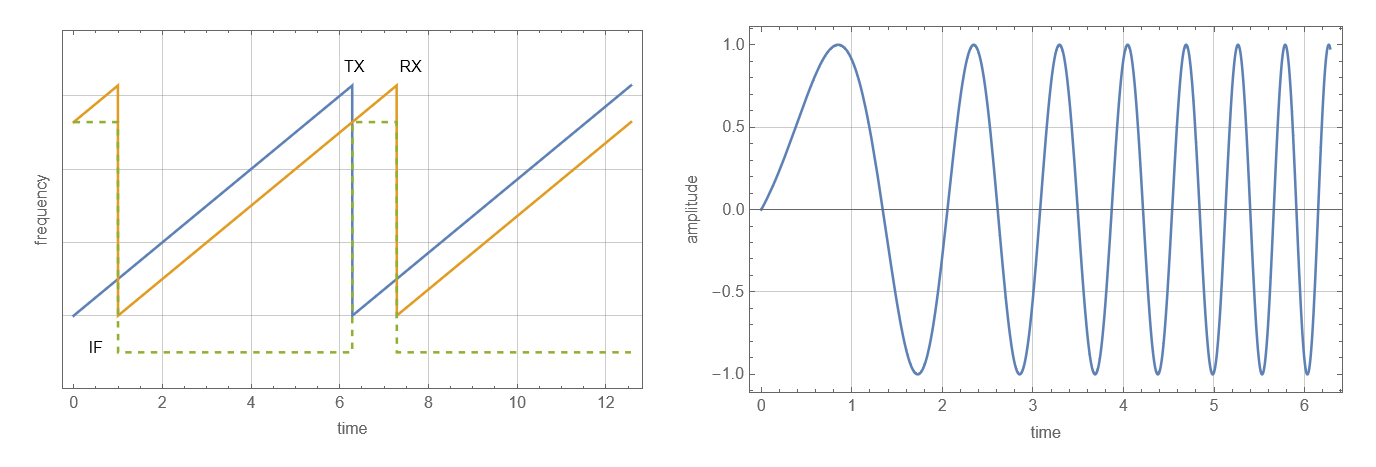
\includegraphics[width=\textwidth]{chirp}
	\caption{Left: transmitted (TX) and received (RX) sawtooth chirps and their difference frequency (IF). Right: illustration of TX chirp waveform.}
	\label{fig:Chirp}
\end{figure}

Frequency-modulated continuous wave (FMCW) radar systems emit consecutive 'chirps' - signals whose frequency is a function of time, often a triangle or sawtooth wave. The reflected chirp arrives at a time \(\Delta t\) after emission, leading to a phase difference as shown in Figure \ref{fig:Chirp}. The transmitted and received signals are passed through a mixer to extract their difference/intermediate frequency (IF).

\paragraph{Range measurement.} The target range relates to the time delay and hence the intermediate frequency by
\begin{equation}
	r = \frac{c \Delta t}{2} = \frac{c f_{IF}}{2} \diff{f}{t}.
\end{equation}
In practice, there are many received signals, thus one performs a discrete Fourier transform of the IF signal to obtain a range profile. The range resolution is limited only by the bandwidth \(B\) of the chirp:
\begin{equation}
	d_{res} = \frac{c}{2B}.
\end{equation}

\paragraph{Velocity measurement.} Velocity data is obtained by analysing the phase of the IF signal \dots

\subsection{Solid state 94-GHz FMCW cloud profiling radar}
The Millimetre Wave and EPR Group at the University of St Andrews has been developing a ground-based, zenith-pointing radar that operates at 94 GHz. \supercite{StAndrewsRadar} The radar utilises solid-state electronics and two Fresnel zone plate antennas, significantly reducing the cost.

\subsubsection{Project work}
The radar software needs to be updated to allow for continuous data output to netCDF files, a format widely used by meteorologists. This data can be processed to obtain reflectivity as a function of height, Doppler velocity moments (mean, skew, kurtosis), among other quantities used by meteorologists.

\subsection{Radar output}
Reflectivity, Doppler velocity (mean, width, skew, kurtosis)
Why are these useful for meteorologists?

\section{Conclusions}

\printbibliography
\end{document}
